\chapter{张量代数}
张量代数在这些地方有出现过:
\begin{enumerate}
\item 理论物理学。
\item 线性代数中的张量积。
\item 范畴论中的共变与反变函子。
\end{enumerate}
从上到下,抽象程序依次提升。这里取中间的一层,即作为多线性代数的张量。

\section{理解张量}
\subsection{理解坐标变换}
\subsubsection{坐标变换与基变换}
坐标变换与基变换,并不完全是一回事。比如用$x_i$表示笛卡尔坐标系的坐标,$\bm{e}^i$表示笛卡尔坐标系的基。给定坐标变换
\begin{empheq}{align*}
x^1&=x_1+x_2\\
x^2&=x_1-x_2-5
\end{empheq}
这是一个平移变换。我们可能设想对应的基变换是直接把坐标换掉:
\begin{empheq}{align*}
	\bm{e}_1&=\bm{e}^1+\bm{e}^2\\
	\bm{e}_2&=\bm{e}^1-\bm{e}^2-5
\end{empheq}
但这是不对的,注意下面一行,左边是向量,而5是常数,相减其实没有定义。而且由于坐标变换中,涉及常数,所以并不能直接用二维笛卡尔基来表示基变换。

\subsubsection{坐标变换的方向}
坐标变换是一个笼统的概念,从函数的角度考虑,一个映射,有定义域与值域的区别,因此在具体的量中进行坐标变换时,也会存在方向的问题。即坐标可以以其它量为参数(是值域),或者是其它量的参数(定义域)。

考虑速度向量,坐标系是$(x^1,x^2,x^3)$,它是时间$t$的函数,则速度向量为
$$(\xi^1,\xi^2,\xi^3)=\left(\odv{x^1}{t},\odv{x^2}{t},\odv{x^3}{t}\right)$$

现在我们有一个新的坐标系$(z^1,z^2,z^3)$,此时使用坐标变换$x^i\rightarrow z^i$,即$x$是$z$的函数,给定$x$,可以求得新坐标$z$。在新坐标系下,速度向量为
\begin{equation}\label{velocity-vector}
\eta^i=\odv{z^i}{t}=\xi^j \pdv{z^i}{x^j}
\end{equation}

新坐标$\bz$在上边,因此速率向量为$(1,0)$张量。

另一方面,又考虑梯度向量。原坐标系也是$(x^1,x^2,x^3)$,函数为$f(x^1,x^2,x^3)$,梯度为
$$\nabla f(x^1,x^2,x^3)=\left(\pdv{f}{x^1},\pdv{f}{x^2},\pdv{f}{x^3}\right)=(\xi^1,\xi^2,\xi^3)$$。现在有一个新坐标系$(z^1,z^2,z^3)$,此时的坐标变换应该为$z^i\rightarrow x^i$,即把$x^i$用$\bz$表示出来,这样才能算出$f$,于是现在新坐标系下
$$\eta_i=\pdv{f}{z^i}=\xi^j\pdv{x^j}{z^i}$$

注意$\eta_i$的下标,对应于$\partial z^i$在下边,因此梯度为$(0,1)$张量。

对比以上两个例子,可以看出,虽然都是坐标变换,但其实方向恰好相反,这种方向上的区别就是协变与共变的区别。然而实际上都是链式法则。

\subsubsection{为什么使用张量}
参考系在物理学中的地位非常重要,同样的物理量,在不同的参考系下有不同的表示。常规情况下,在一个坐标系下进行计算的结果,在新坐标系下,需要重新计算一遍:
\begin{center}
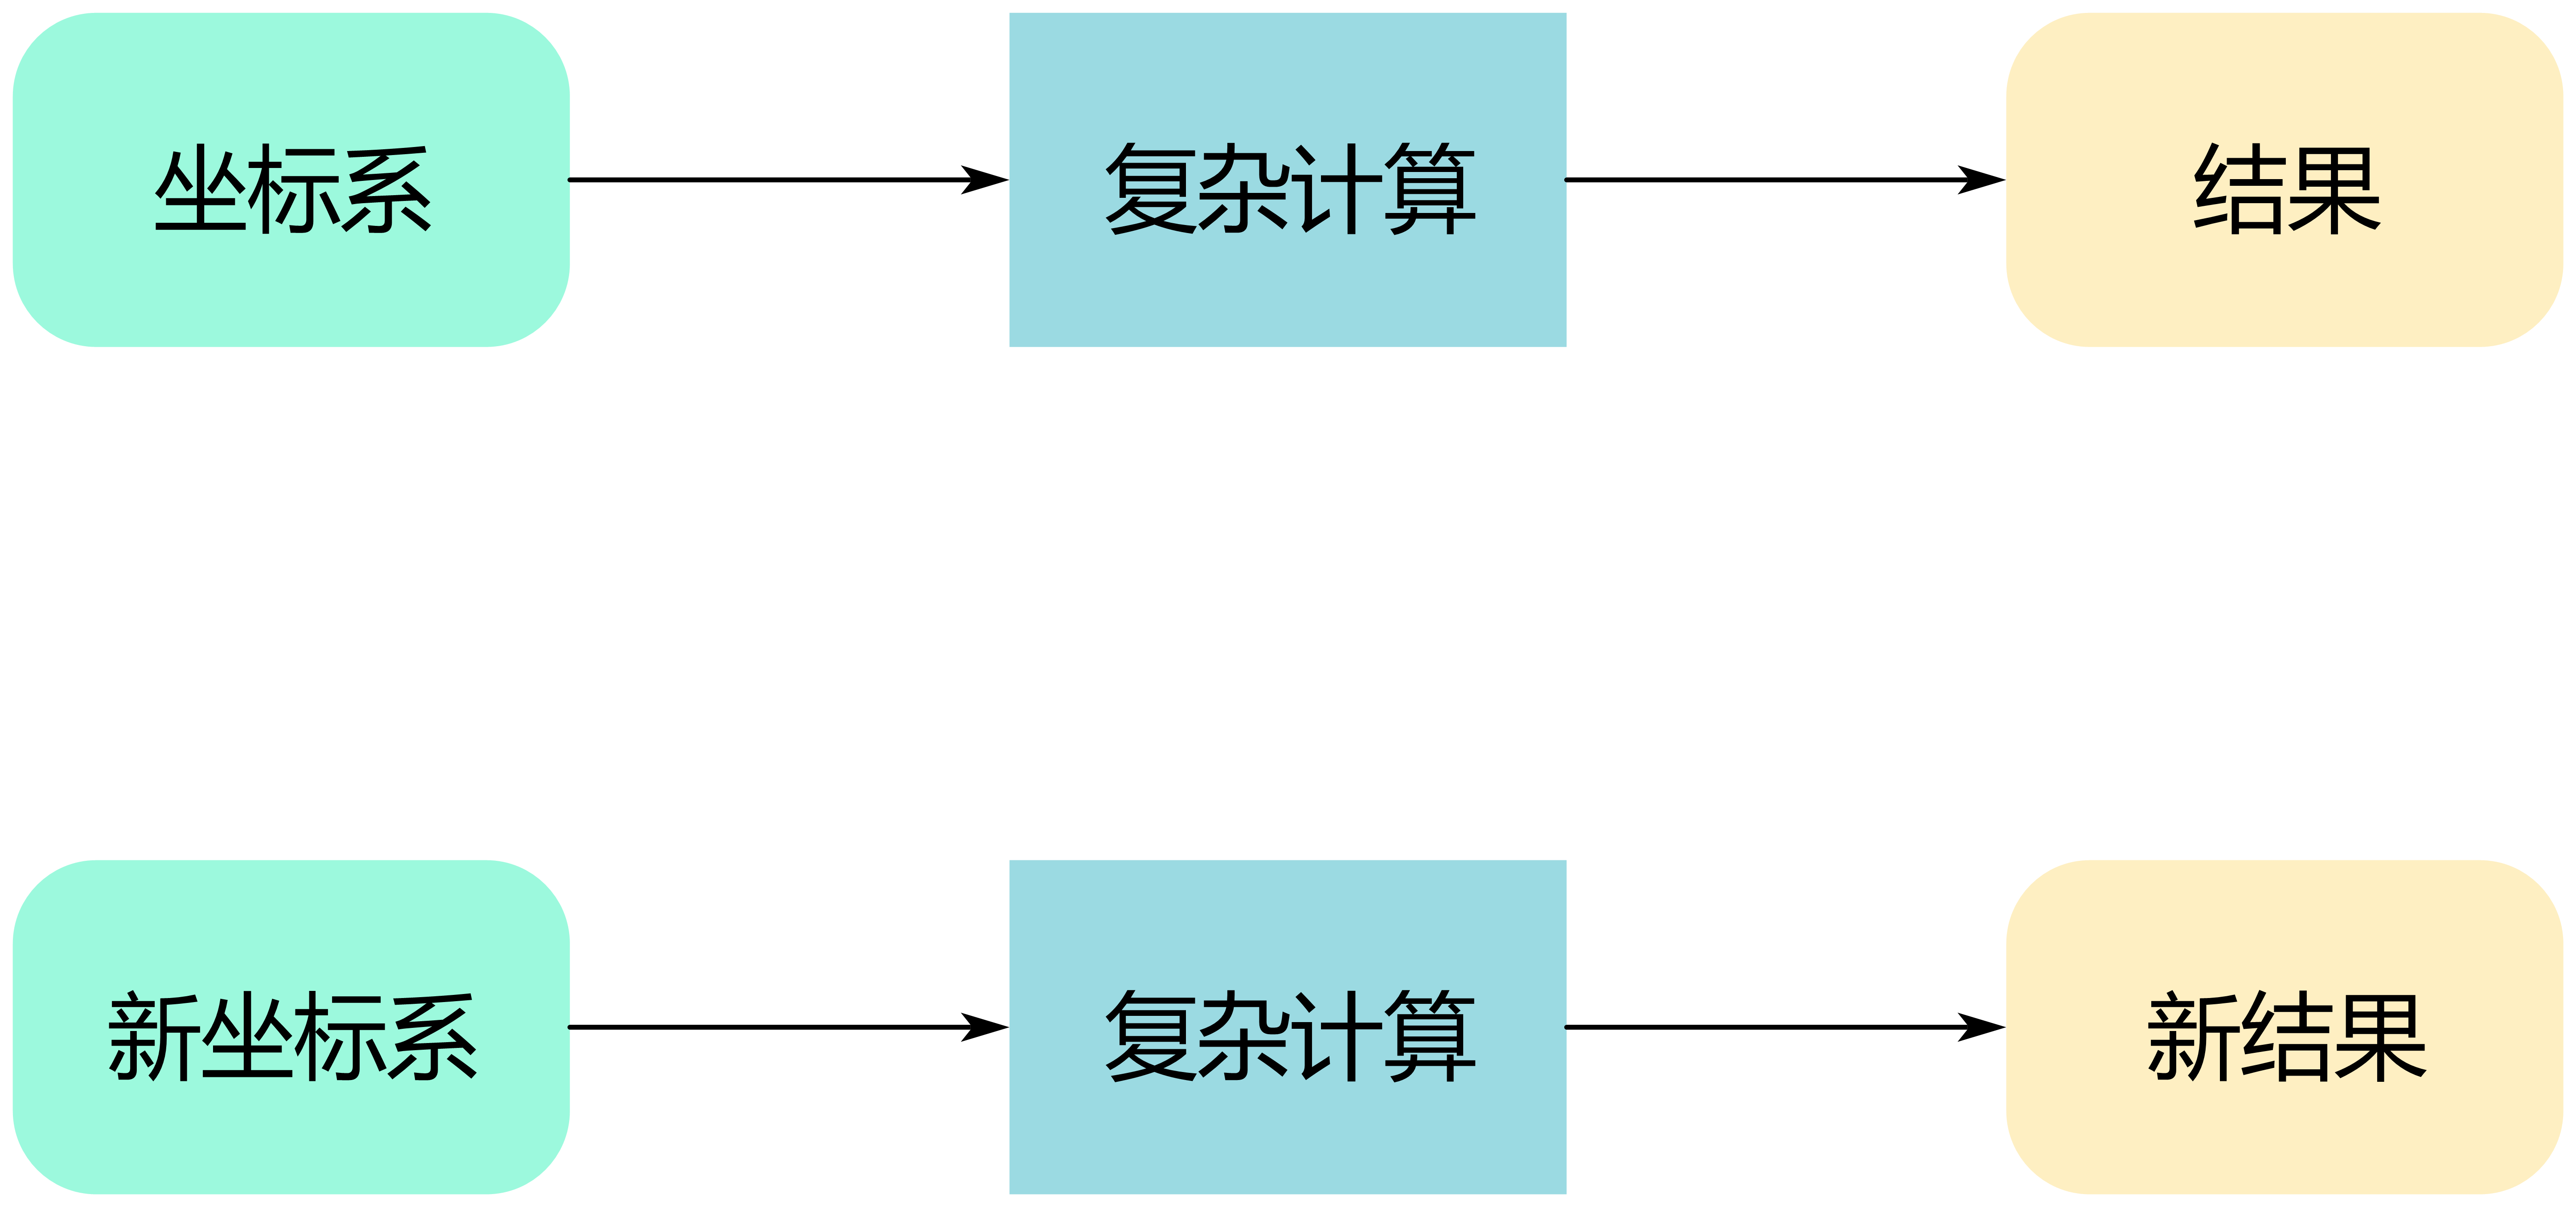
\includegraphics[width=8cm]{figure/NoTensor.png}
\end{center}
这样是非常繁琐的,而且不同的坐标系是无限多的。

现在引入张量,张量就是在坐标变换下不变的量。张量本身在不同的坐标系下是不变的,但张量在不同坐标系下的表示却是不同的。有了张量,我们就只需要在一个坐标系下进行计算,得出结果,然后找出坐标变换,对结果也进行一下坐标变换,就得到了在新坐标系下的结果,不需要重行进行计算:
\begin{center}
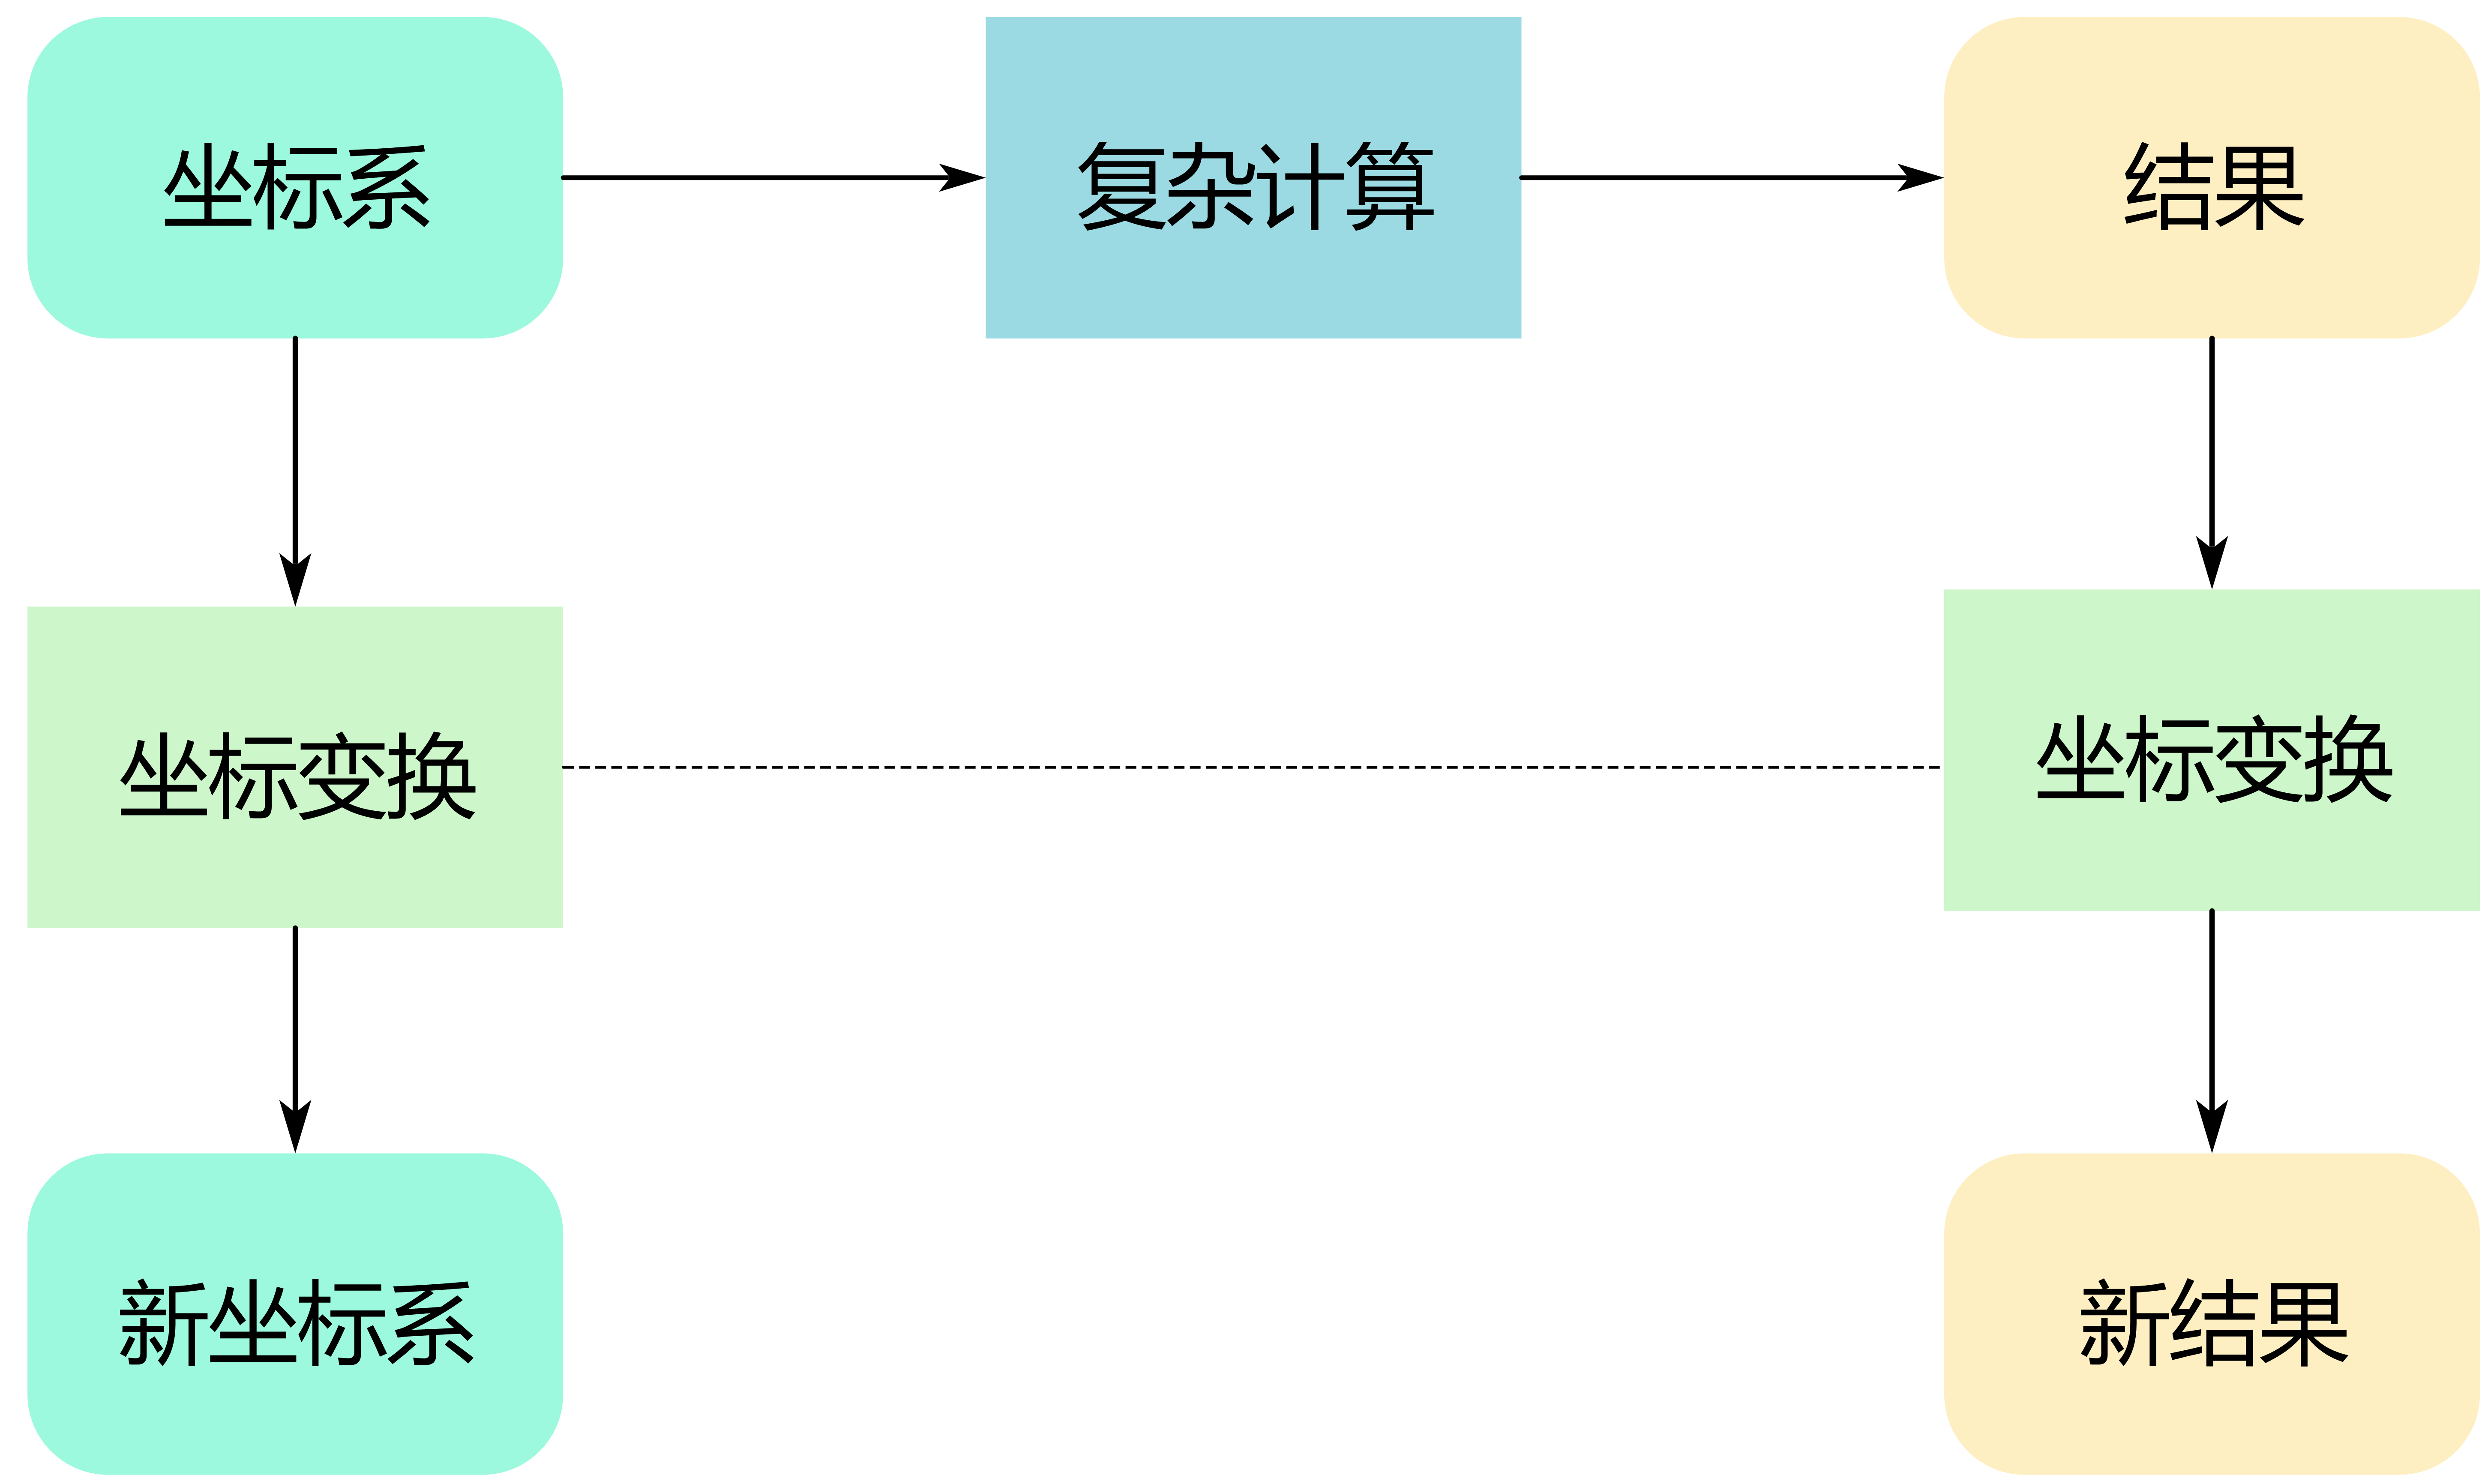
\includegraphics[width=8cm]{figure/WithTensor.png}
\end{center}
\subsection{协变与逆变(或共变与反变)}
在线性代数中,记$E$的列$\{\bm{e}_1,\cdots,\bm{e}_n\}$为某个坐标系下的基,则给定坐标变换
$$E'=ET$$
$T$称为从基$\{\bm{e}_1,\cdots,\bm{e}_n\}$到基$\{\bm{e}_1',\cdots,\bm{e}_n'\}$的过渡矩阵。

假设在某个坐标系$E$下,某个欧几里得空间中的向量表示为$\bx$,那么在基变换$T$下有$E'=ET$,由于张量是不变的,所以
\[
\begin{aligned}
E'\bx'&=E\bx\\
ET\bx'&=E\bx\\
x'&=T^{-1}x
\end{aligned}
\]

注意到坐标变换式与基变换式恰好相反,所以欧几里得空间中的张量是一次反变张量。

我们说的反变与共变张量是指张量在坐标变换下的性质。似乎与反变分量、共变分量并不完全一样,说反变、共变分量时,一定是针对基与对偶基而言的,而基与对偶基(reciporical basis)之间需要满足某种关系,并不能随意选取。关于反变与共变分量需要记住:
\begin{center}
\textbf{张量在共变基下的分量叫反变分量。}\\
\textbf{张量在反变基下的分量叫共变分量。}
\end{center}
这里可以看出,爱因斯坦求和是对上指标与下指标求和。

$(p,q)$型张量称为$p$次反变($p$个反变基)、$q$次共变($q$个共变基)张量,表示为$T^p_q(V)$,可见上标是反变,下标是共变。


\subsection{张量的例子}

\section{Einstein记号与张量乘法}
\subsection{多维数组的Einstein记号}
以下用$A_{ij}$来表示一个二维数组。使用Einstein记号可以很方便地表示多维数组的乘法和一些运算:
\subsubsection{矩阵运算}
\begin{empheq}{align}
AB&=Y_{ij}=A_{ik}B_{kj} \mtag{矩阵乘法}\\
ABC&=Y_{ij}=A_{ik}B_{kl}C_{lj}\\
ABCD&=Y_{ij}=A_{ik}B_{kl}C_{lm}D_{mj}\\
A^TA&=Y_{ij}=A_{ki}A_{kj}\\
XA^TAX^T&=Y_{ij}=X_{ik}A_{lk}A_{lm}X_{jm}\\
\bx^TA\by&=L=x_iA_{ij}y_j
\end{empheq}
以下用$[\underline{\bx^T}_m]$表示把一个行向量沿行方向复制多份,构成矩阵。$A\odot [\underline{\bx^T}_m]$就是把矩阵$A$的每一行按元素乘以$\bx$。
\begin{empheq}{align}
A\odot [\underline{\bx^T}_m] &=Y_{ij}=A_{ij}x_j
\end{empheq}
\begin{empheq}{align}
\trace(A)&=L=A_{ii}\\
\trace(AB)&=L=A_{ik}B_{ki}\\
\trace(XAX^T)&=L=X_{ik}A_{kl}X_{li}\\
\trace(XA^TAX^T)&=L=X_{ik}A_{lk}A_{lm}X_{im}
\end{empheq}
\begin{empheq}{align}
\diag(A)&=\bx_{i}=A_{ii}\\
\diag(AB)&=\bx_{i}=A_{ij}B_{ji}
\end{empheq}
\section{张量的定义}
\subsection{$(p,q)$型张量}
\begin{definition}[$(p,q)$型张量]{}
称在坐标系$(x^1,\cdots,x^n)$下给出的数组$T^{i_1\cdots i_p}_{j_1\cdots j_q}$为$p+q$阶的$(p,q)$型张量是指它按如下方式在依赖于坐标系:

$$T^{i_1\cdots i_p}_{j_1\cdots j_q}=\sum_{k,l}{T'}^{k_1\cdots k_p}_{l_1\cdots l_q}\pdv{x^{i_1}}{z^{k_1}}\cdots\pdv{x^{i_p}}{z^{k_p}}\pdv{z^{l_1}}{x^{j_1}}\cdots\pdv{z^{l_q}}{x^{j_1}}$$
\end{definition}
以之前的速度向量\eqref{velocity-vector}为例,在$\bz$坐标系下,其表示式中$\partial z^i$在上边,因此就是$(1,0)$型张量。